% \subsection {Algorithm Overview}

\begin{figure}
\begin{center}
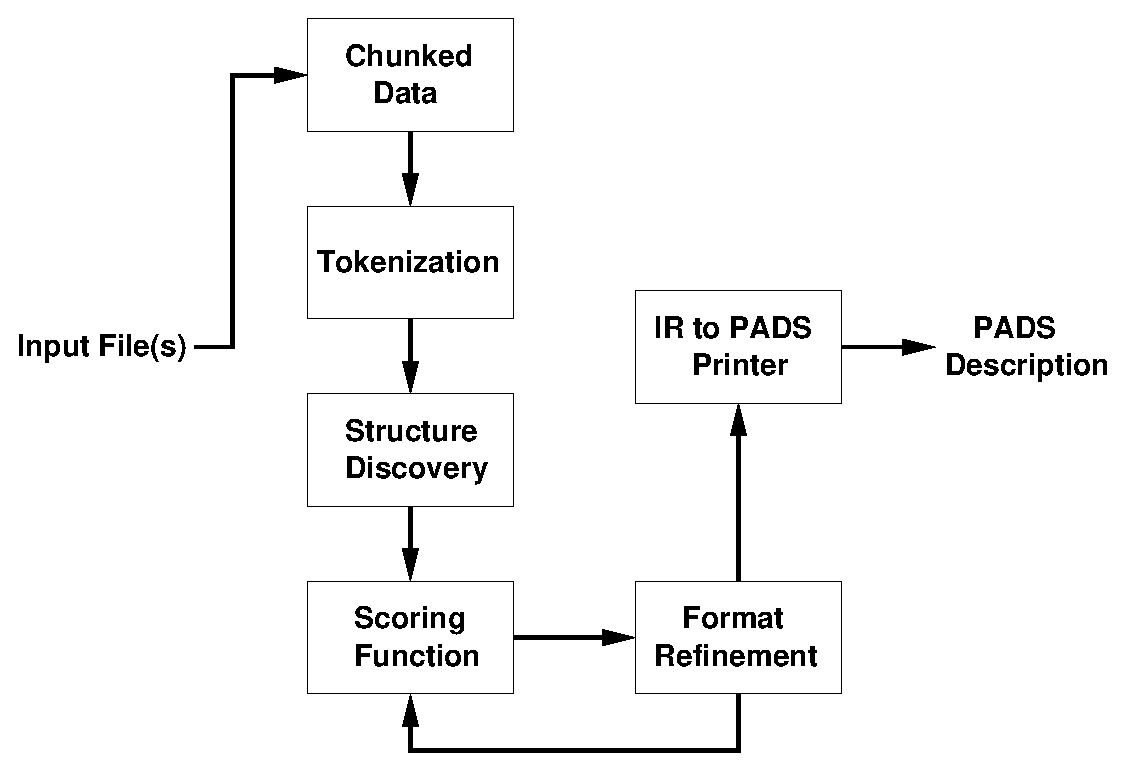
\epsfig{file=archi.eps, width=.9\columnwidth}
\caption{Architecture of the format inference engine}
\vspace*{-5mm}
\label{fig-archi}
\end{center}
\end{figure}

Figure \ref{fig-archi} gives an overview of our format inference
architecture. The input data ({\em i.e.,} training set) is first
divided into {\em chunks} as specified by the user.  Intuitively, a chunk
is a unit of repetition in the data source.  Our tool currently supports
chunking on a line-by-line basis as well as on a file-by-file basis.  

Each chunk is broken down into a
series of {\em tokens} by a lexer.
Each token can be a punctuation symbol, a
number, a date, a time, or a number of other basic items.  Every token
type has a corresponding base type in the \ir{}, though the 
converse is not true -- there are
a number of base types that are not used as tokens.

Our learning system has a default tokenization scheme skewed toward systems
data, but users may specify a different scheme for their own domain
through a configuration file.  For example, computational biologists
may want to add DNA strings {\tt CATTGTT...} to the default tokenization 
scheme.  The configuration file is essentially
a list of name-regular expressions pairs -- see Figure~\ref{fig:configfile}
for a small example.  The system uses the file to generate 
part of the system's lexer, a
collection of new \ir{} base types, and a series of type 
definitions that are incorporated into the final \pads{} specification.  

After tokenization, the algorithm enters the {\em structure discovery} 
phase.  This phase uses a top-down, divide-and-conquer
scheme to guess an approximate, initial format for the data.
To assess the quality of this initial approximation, the
algorithm computes an information-theoretic {\em score} for the
structure.  This score is used in the next phase to guide
{\em rewriting rules} that iteratively refine the format.  

Once the format has been refined to the extent possible, the resulting
\ir{} is printed in \pads{} syntax.  Template programs that use the
new description, including the \xml{}-converter, a simple
statistics tool we call the {\em accumulator}, a database tool
based on Oetiker's RRDTool~\cite{rrdtool}, and the \padx{}
query engine, are also all generated at this point.  Hence, starting
with data alone, our end-to-end algorithm quickly generates an entire suite
of fully functional data processing tools, ready to use at the command line.

The following subsections describe the main components of the algorithm
in more detail, including the structure discovery phase, the 
information-theoretic scoring function, the structure refinement phase
and the end products of the algorithm.

\begin{figure}
\begin{verbatim}
def triplet [0-9]{1,3}
def doublet [0-9]{1,2}
def hexdoub [0-9a-fA-F]{2}
...
exp Pemail {str1}@{hostname}
exp Pmac   ({hexdoub}(: | \-)){5}{hexdoub}
exp PbXML  \<([a-zA-Z])+\>
exp PeXML  \<\/[^>]+\>
\end{verbatim}
\caption{Tiny fragment of the default configuration file. 
The configuration command {\tt exp} specifies the definition on that
line should be  ``exported'' to
the learning tool whereas command {\tt def} implies the definition
is local and used only in other {\tt exp} or {\tt def} in the
configuration file.}
\label {fig:configfile}
\end{figure}

%% \subsection {Chunking and Tokenization}




%% \begin{figure}
%% \begin{center}
%% \begin{tabular}{|l|l|}
%% \hline
%% Name   &  Description               \\ \hline\hline
%% Pint  &   Integer \\ 
%% Palpha & Alpha-numeric string including '$\_$' and '$-$' \\
%% Pip & IP address \\
%% Pemail & Email address \\
%% Pmac & Mac address \\
%% Pdate & Simple date format \\
%% Ptime & Simple time format \\
%% Ppath & File system path \\
%% Phostname & Hostname \\
%% Purl  & URL \\
%% PbXML & Beginning XML tag \\
%% PeXML & Ending XML tag \\
%% Pother & Punctuation character \\\hline
%% \end{tabular}

%% \caption{Basic token types in default configuration.}
%% \label{figure:base-types}
%% \end{center}
%% \end{figure}
 



%%     *  mention system parameterization for multiple tokenizations for different domains
%%     * mention current skew towards systems data
%%     * ignore problems in this section -- save that for discussion/future work section
%%     * mention stream of tokens generated for running example 

\subsection {Structure Discovery}

Inspired in part by the work of Arasu on
information extraction from web pages~\cite{arasu+:sigmod03}. 

    *  role = quickly find a description in the "approximate area" of the correct description
    * explain structure of a generic "top-down" inference algorithm -- perhaps give pseudocode
    * explain our heuristics: generation of histograms, choice of struct, array, union, base type
    * grouping construct (introduce additional example as needed)
    * show (part of?) description of running example 

\subsection {Information-Theoretic Scoring}

    *  role = evaluate the "goodness" of the description relative to data
    * explain the information-theoretic principles
    * give the formulas 

\subsection {Structure Refinement}

%\documentclass[fleqn]{article}
\usepackage{code}
\newcommand{\struct}[1]{{\tt struct}\{#1\}}
\newcommand{\union}[1]{{\tt union}\{#1\}}
\newcommand{\enum}[1]{{\tt enum}\{#1\}}
\newcommand{\parray}[1]{{\tt array}\{#1\}}
\newcommand{\arrayFW}[2]{{\tt arrayFW}\{#1\}[#2]}
\newcommand{\switch}[2]{{\tt switch}(#1)\{#2\}}
\newcommand{\option}[1]{{\tt option}\{#1\}}
\newcommand{\goto}{\Rightarrow}
\begin{document}
\section{Rewriting Rules}
\subsection*{Data independent rules}
\begin{enumerate}
\item Singleton structs and unions.
\[
\struct{T} \goto T
\]
\[
\struct{} \goto \bot 
\]
\[
\union{T} \goto T
\]
\[
\union{} \goto \bot 
\]

\item Struct and union clean-up
\[
\struct{T_1; \ldots; T_i; \bot; T_j; \ldots; T_n} \goto
\struct{T_1; \ldots; T_i; T_j; \ldots; T_n} 
\] 
\[
\struct{T_1; \ldots; T_i; \emptyset; T_j; \ldots; T_n} \goto
\struct{T_1; \ldots; T_i; T_j; \ldots; T_n} 
\] 

\[
\union{T_1; \ldots; T_i; \bot; T_j; \ldots; T_n} \goto
\union{T_1; \ldots; T_i; T_j; \ldots; T_n} 
\] 
\[
\union{T_1; \ldots; T_i; \emptyset; T_j; \ldots; T_n} \goto
\union{T_1; \ldots; T_i; T_j; \ldots; T_n; \emptyset} 
\]
\noindent where $\emptyset$ means {\tt Pempty}.

\item Union to option
\[
\union{T; \emptyset} \goto \option{T}
\]
\[
\union{\emptyset; T} \goto \option{T}
\]

\item Unnest structs and unions
\begin{eqnarray*}
&& \struct{pretypes; \struct{T_1; \ldots; T_n}; posttypes} \goto \\
&& \struct{pretypes; T_1; \ldots; T_n; posttypes}
\end{eqnarray*}
\begin{eqnarray*}
&&\union{pretypes; \union{T_1; \ldots; T_n}; posttypes} \goto \\
&&\union{pretypes; T_1; \ldots; T_n; posttypes}
\end{eqnarray*}

\item Uniform struct to fixed-length array
\[
\struct{T_1; \ldots; T_n} \goto \arrayFW{T_1}{n}
\]
\noindent if $T_1 = \ldots = T_n$ and $n>=3$.

\item Common prefix or postfix in union branches
\begin{eqnarray*}
&&\union{\struct{T; posttypes_1}; \struct{T, posttypes_2}} \goto \\
&&\struct{T; \union{\struct{posttypes_1}; \struct{posttypes_2}}}
\end{eqnarray*}
\begin{eqnarray*}
&&\union{\struct{T; posttypes}; T} \goto \\
&&\struct{T; \union{\struct{posttypes}; \emptyset}}
\end{eqnarray*}
\begin{eqnarray*}
&&\union{\struct{pretypes_1; T}; \struct{pretypes_2; T}} \goto \\
&&\struct{\union{\struct{pretypes_1}; \struct{pretypes_2}}; T}
\end{eqnarray*}
\begin{eqnarray*}
&&\union{\struct{pretypes; T}; T} \goto \\
&&\struct{\union{\struct{pretypes}; \emptyset}; T}
\end{eqnarray*}

\item {Get floating number number}
\[
\union{{\tt Pint}; {\tt Pfloat}} \goto {\tt Pfloat}
\]

\end{enumerate}

\subsection*{Data dependent rules}
\begin{enumerate}
\item Get floating point number
\begin{eqnarray*}
&& \struct{pretypes; {\tt Pint}(x); {\tt PstringConst ('.')}; {\tt Pint}(y); posttypes} \goto \\
&& \struct{pretypes; {\tt Pfloat}; posttypes}
\end{eqnarray*}
\noindent if $y \ge 0$.
\begin{eqnarray*}
&& \struct{pretypes; {\tt Pint}(x); \option{\struct{{\tt PstringConst ('.')}; {\tt Pint}(y)}}; posttypes} \goto \\
&& \struct{pretypes; {\tt Pfloat}; posttypes}
\end{eqnarray*}
\noindent if $y \ge 0$.

\item Discover negative numbers
\begin{eqnarray*}
&& \struct{pretypes; {\tt Pother}; {\tt PstringConst}('-'); {\tt Pint}(x); posttypes} \goto \\
&& \struct{pretypes; {\tt Pother}; {\tt Pint}; posttypes}
\end{eqnarray*}
\noindent if $x \ge 0$.
\begin{eqnarray*}
&& \struct{pretypes; {\tt Pother}; {\tt PstringConst}('-'); {\tt Pfloat}(x); posttypes} \goto \\
&& \struct{pretypes; {\tt Pother}; {\tt Pfloat}; posttypes}
\end{eqnarray*}
\noindent if $x \ge 0$.
\begin{eqnarray*}
&& \struct{pretypes; {\tt Pother}; \option{{\tt PstringConst}('-')}; {\tt Pint}(x); posttypes} \goto \\
&& \struct{pretypes; {\tt Pother}; {\tt Pint}'; posttypes}
\end{eqnarray*}
\noindent if $x \ge 0$.
\begin{eqnarray*}
&& \struct{pretypes; {\tt Pother}; {\tt \option{PstringConst}('-')}; {\tt Pfloat}(x); posttypes} \goto \\
&& \struct{pretypes; {\tt Pother}; {\tt Pfloat}'; posttypes}
\end{eqnarray*}
\noindent if $x \ge 0$.

\item Unique base types to constant
\[
{\tt Pint}(x) \goto {\tt PintConst(c)}~~ {\rm if}~~ x = c.
\]
\[
{\tt Palpha}(x) \goto {\tt PstringConst(c)}~~ {\rm if}~~ x = c.
\]
\[
{\tt Pstring}(x) \goto {\tt PstringConst(c)}~~ {\rm if}~~ x = c.
\]
\[
{\tt Pother}(x) \goto {\tt PstringConst(c)}~~ {\rm if}~~ x = c.
\]


\item Combine adjacent constant strings
\begin{eqnarray*}
&& \struct{pretypes; {\tt PstringConst (c_1)}; {\tt PstringConst(c_2)}; posttypes} \goto \\
&& \struct{pretypes; {\tt PstringConst (c_1 + c_2)}; posttypes} 
\end{eqnarray*}

\item Refine enums and ranges
\[
{\tt Pstring}(x) \goto \enum{s_1; \ldots; s_k} ~~
{\rm if}~ x~ \in \{s_1, \ldots, s_l\}.
\]
\[
{\tt Pint}(x) \goto {\tt Pint32} ~~
{\rm if}~ 0 \le x~ < 2^{32}.
\]
\[
{\tt Pint}(x) \goto {\tt Pint64} ~~
{\rm if}~ 2^{32} \le x~ < 2^{64}.
\]

\[
{\tt Pint}(x) \goto {\tt PintRanged}(min,~ max) ~~
{\rm if}~ min \le x~ \le max.
\]
\item Union to switch
\begin{eqnarray*}
&&\struct{pretypes; b(x); midtypes; \union{T_1; \ldots; T_n}; posttypes} \goto \\
&&\struct{pretypes, b(x); midtypes; \switch{x}{s_1 \goto T_1; \ldots; s_n \goto T_n}; posttypes}
\end{eqnarray*}
\noindent where $\forall i \in [i,~ n],~ inj_i(\union{T_1; \ldots; T_n}) {\rm implies}~ x = s_i$.

\end{enumerate}

\end{document}


    *  role = starting with the candidate structure, search for nearby descriptions that optimize an information theoretic scoring function
    * explain the 3 parts: value independent, value dependent, value independent
    * give (partial) list of rules used -- we need to work on notation for explaining these rules
    * illustrate several transformations using the running example
    * compare example after rewriting to the example from subsection 3.4 above
    * optional subsubsection: theory suggesting our algorithm is "correct" (we'd need a semantics for our IR then)

\subsection*{Data independent rules}
$T_{punc}$ is any type that describes a punctuation or white space.
$T\setof{X}$ means a type $T$ where $X$ is a {\em bag} of data representations
parsed by $T$.

\begin{enumerate}
\item Singleton structs and unions. \\
$
\irstruct{T} \goto T
$\\ \\
$
\irstruct{} \goto \Pempty
$\\ \\
$
\irunion{T} \goto T
$\\ \\
$
\irunion{} \goto \Pvoid 
$\\ \\

\item Struct and union clean-up\\
$
\irstruct{pre\_types; \Pvoid; post\_types} \goto \Pvoid
$\\ \\ 
$
\irstruct{pre\_types; \Pempty; post\_types} \goto \\
\sskip \irstruct{pre\_types; post\_types}
$\\ \\ 
$
\irunion{pre\_types; \Pvoid; post\_types} \goto \\
\sskip \irunion{pre\_types; post\_types} 
$\\ \\
$
\irunion{pre\_types; \Pempty; post\_types} \goto \\
\sskip \irunion{pre\_types; post\_types; \Pempty} 
$\\ \\

\item Union to option\\
$
\irunion{T; \Pempty} \goto \iroption{T}
$\\ \\
$
\irunion{\Pempty; T} \goto \iroption{T}
$\\ \\

\item Unnest structs and unions\\
$
\irstruct{pre\_types; \irstruct{mid\_types}; post\_types} \goto \\
\sskip \irstruct{pre\_types; mid\_types; post\_types}
$\\ \\
$
\irunion{pre\_types; \irunion{mid\_types}; post\_types} \goto \\
\sskip \irunion{pre\_types; mid\_types; post\_types}
$\\ \\

\item Uniform struct to fixed-length array\\
$
\irstruct{T_1; \ldots; T_n} \goto \irarrayFW{T_1}{n}
$\\ 
\noindent if $n \ge 3$ and $\forall i \in [1,~ n],~ j \in [1,~ n]:~ T_i = T_j$.
\\

\item Common prefix or postfix in union branches \\
$
\irunion{\irstruct{T; post\_types_1}; \\
\sskip \irstruct{T, post\_types_2}} \goto \\
\sskip \irstruct{T; \irunion{\irstruct{post\_types_1}; \\
\sskip \irstruct{post\_types_2}}}
$\\ \\
$
\irunion{\irstruct{T; post\_types}; T} \goto\\
\sskip \irstruct{T; \irunion{\irstruct{post\_types}; \Pempty}}
$\\ \\
$
\irunion{\irstruct{pre\_types_1; T}; \\
\sskip \irstruct{pre\_types_2; T}} \goto \\
\sskip \irstruct{\irunion{\irstruct{pre\_types_1}; \\
\sskip \irstruct{pre\_types_2}}; T}
$\\ \\
$
\irunion{\irstruct{pre\_types; T}; T} \goto \\
\sskip \irstruct{\irunion{\irstruct{pre\_types}; \Pempty}; T}
$\\ \\

\item {Get floating number number}\\
$
\irunion{{\tt Pint}; {\tt Pfloat}} \goto {\tt Pfloat}
$ 
\end{enumerate}

\subsection*{Data dependent rules}
\begin{enumerate}
\item Get floating point number \\
$
\irstruct{pre\_types; {\tt Pint}\setof{X}; {\tt PstringConst ('.')};  \\
\sskip {\tt Pint}\setof{Y}; post\_types} \goto \\
\sskip \irstruct{pre\_types; {\tt Pfloat}; post\_types}
$\\ 
\noindent if $\forall y \in Y:~ y \ge 0$. \\
\\
$
\irstruct{pre\_types; {\tt Pint}\setof{X}; \\
\sskip \iroption{\irstruct{{\tt PstringConst ('.')};  \\
\sskip {\tt Pint}\setof{Y}}}; post\_types} \goto \\
\sskip \irstruct{pre\_types; {\tt Pfloat}; post\_types}
$ \\
\noindent if $\forall y \in Y:~ y \ge 0$. \\

\item Discover negative numbers\\
$
\irstruct{pre\_types; T_{punc}; {\tt PstringConst}('-');\\
\sskip {\tt Pint} \setof{X}; post\_types} \goto \\
\sskip \irstruct{pre\_types; T_{punc}; {\tt Pint}; post\_types}
$\\ 
\noindent if $\forall x \in X:~ x \ge 0$. \\
\\
$
 \irstruct{pre\_types; T_{punc}; {\tt PstringConst}('-'); \\
\sskip {\tt Pfloat}\setof{X}; post\_types} \goto \\
\sskip \irstruct{pre\_types; T_{punc}; {\tt Pfloat}; post\_types}
$\\ 
\noindent if $\forall x \in X:~ x \ge 0$.\\
\\
$
 \irstruct{pre\_types; T_{punc}; \iroption{{\tt PstringConst}('-')}; \\
\sskip {\tt Pint}(x); post\_types} \goto \\
\sskip \irstruct{pre\_types; T_{punc}; {\tt Pnat}; post\_types}
$\\
\noindent if $\forall x \in X:~ x \ge 0$.\\
\\
$
\irstruct{pre\_types; T_{punc}; {\tt \iroption{PstringConst}('-')}; \\
\sskip {\tt Pfloat}(x); post\_types} \goto \\
\sskip  \irstruct{pre\_types; T_{punc}; {\tt Preal}; post\_types}
$\\
\noindent if $\forall x \in X:~ x \ge 0$.\\

\item Base type with unique values to constant \\
$
{\tt Pint}\setof{X} \goto {\tt PintConst(c)} \\
$
{\rm if} $\forall x \in X:~ x = c$. 
\\ \\
$
{\tt Palpha}\setof{X} \goto {\tt PstringConst(c)} \\
$
{\rm if} $\forall x \in X:~ x = c$.
\\ \\
$
{\tt Pstring}\setof{X} \goto {\tt PstringConst(c)} \\
$
{\rm if} $\forall x \in X:~ x = c$.
\\ \\
$
{\tt Pother}\setof{X} \goto {\tt PstringConst(c)} \\ 
$
{\rm if} $\forall x \in X:~ x = c$.
\\ \\

\item Combine adjacent constant strings \\
$
\irstruct{pre\_types; {\tt PstringConst (c_1)}; \\
\sskip {\tt PstringConst(c_2)}; post\_types} \goto \\
\sskip \irstruct{pre\_types; {\tt PstringConst (c_1 \wedge c_2)}; post\_types} 
$\\ \\

\item Refine enums and ranges \\
$
{\tt Pstring}\setof{X} \goto \irenum{s_1; \ldots; s_k} \\
$
{\rm if}~ $\forall x \in X:~ x~ \in \{s_1, \ldots, s_k\}$.
\\ \\
$
{\tt Pint}\setof{X} \goto {\tt Pint32} \\
$
{\rm if} $\forall x \in X:~ 0 \le x~ < 2^{32}$.
\\ \\
$
{\tt Pint}\setof{X} \goto {\tt Pint64} \\
$
{\rm if} $\forall x \in X:~ 2^{32} \le x~ < 2^{64}$.
\\ \\
$
{\tt Pint}\setof{X} \goto {\tt PintRanged}(min,~ max) \\
$
{\rm if}~ $\forall x \in X:~ min \le x~ \le max$.
\\ \\

\item Union to switch \\
$
\irstruct{pre\_types; \irenum{c_1; \ldots; c_n}\setof{X}; mid\_types; \\
\sskip \irunion{T_1; \ldots; T_n}\setof{Y}; post\_types}\\
\goto \\
\irstruct{pre\_types, z:\irenum{c_1; \ldots; c_n}; mid\_types; \\
\sskip \irswitch{z}{c_1 \goto T_{\Pi(1)}; \ldots; c_n \goto T_{\Pi(n)}}; post\_types}
$\\ 
\noindent where $z$ is a fresh variable, and there exists a permutation $\Pi$, s.t.
$\forall i \in [1,~ card(X)]$, $\Pi(tag(X(i)))=tag(Y(i))$, and 
$tag(in_j(d)) = j$.

\end{enumerate}
 

\subsection {Finishing Up}

    * printing pads syntax and invoking toolchain
